\chapter{Experimental Techniques}

In the previous chapter we provided a microscopic description of ferromagnetism and the motivation for how certain properties of ferromagnets arise. In this section, we will proceed to treat the interaction of light with these properties and explain how light can be used as a sensitive probe for magnetism. 

Although visible light interacts with magnetism in materials in a non-resonant fashion, the resonant interaction of high energy light with the core level electrons in a ferromagnet provides a much stronger and more detailed source of information about the material. Traditionally, the 2p core level shells have been probed using light from synchrotrons and free electron lasers. The physics that describes these resonances is almost identical to the physics that occurs when light resonant at the 3p level shells is used. In this thesis, we generate light resonant with the 3p level electrons via the process of high harmonic generation. This technique has the advantages that the temporal duration of the probe is $<$ 10 fs and carries a broad comb of energies, that can be resonant with multiple chemical elements simultaneous. 

The resonance associated with the 3p core level electrons in transition metals is commonly referred to as the M-edge, while the 2p level resonance is called the L-edge. In this section, we will explain how the resonance at the L-edge can be used to directly measure the magnetic moment of a material. This description also applies to light resonant at the M-edges. Additionally, we will focus on circularly polarized light, because it provides an intuitive and convenient basis for our discussion. However, all of the experiments performed in this thesis were in fact carried out using linearly polarized light. This is possible because linear polarization is also a combination of right and light circularly polarized light, and for certain geometries, the microscopic physics that we will discuss here leads directly to a complex dielectric permittivity tensor that interacts with linearly polarized light in a useful fashion.

Erskine and Stern (cite 1975) first proposed the use of X-rays resonant with the core level to valence band transitions to measure magneto-optical properties in the transition metals. The first X-ray magneto-optical effects were then discovered in 1986 and 1987 (Laan and Schutz).

\section{Resonant processes in magnetic materials: determining the X-ray absorption intensity}

In this thesis, two different resonant processes are used to monitor fundamental changes in magnetic materials after ultrafast laser excitation. The first is to directly monitor the charge response using the change in absorption of the resonant extreme ultraviolet light, and the second is to monitor the change in magnetic moment using the magneto-optical Kerr effect. In this section, we theoretically derive the origin for each of these effect, starting the sum rule for charges and how the absorption intensity for a transition from a core to valence band depends directly on the number of holes in the valence band. Using this information it is a straightforward extension to see how circularly polarized light is also sensitive to the number of spin up and spin down electrons in the valence band as well. This information can then be used to monitor the magnetic moment of the material and is the fundamental basis for the magneto-optical effects employed in this thesis.

\subsection{Transition matrix element for atoms}

We begin from the most basic quantum mechanical expression available to describe polarization dependent X-ray absorption and resonant scattering. We want to calculate the intensity of a strong resonance such as the 2$p_{3/2}$,2$p_{1/2}\rightarrow3d$ transition.

The transition matrix elements can be written (by quantizing the electromagnetic field) in the general form:

\begin{equation}
M = \braket{b| \pmb{p}\cdot \pmb{\epsilon} e^{ik\cdot r}|a}
\end{equation}
with p the electron momentum vector, $\epsilon$ the unit photon polarization vector, and k the photon wave vector. We can simplify this expression by taking the dipole approximation, which is well justified in both the soft x-ray (L-edge) and extreme ultraviolet (M-edge) regimes. This is simply the assumption that size of the absorbing atomic shell is small relative to the X-ray wavelength, so that the electric field that drives the electronic transition is constant over the atomic volume. In the photon energy range $\hbar\omega\leq$ 1,000 eV, with a wavelength $\lambda>1.2$ nm with transitions from the 2p core shell of radius $|r|$ $\approx$0.01 nm so that $|r|$ $\approx$0.01 nm $<$ $\lambda/2\pi\approx$0.2 nm. Given that the wavelength of EUV is an order of magnitude larger, while the 3p shell is only marginally larger in spatial extent to the 2p shell, it is reasonable to use the dipole approximation for our discussion here. In this approximation we have:

\begin{equation}
M = \braket{b|\pmb{p}\cdot\pmb{\epsilon}(1+ik\cdot r + \dots)|} \approx \braket{b|\pmb{p}\cdot \pmb{\epsilon} |a} = i m_e \omega \braket{b|\pmb{r} \cdot \pmb{\epsilon} |a}
\end{equation}
with $m_e$ the electron rest mass, and $\omega=\omega_b-\omega_a$ the photon frequency for the transition from state $\ket{a}$ to state $\ket{b}$. The X-ray absorption cross section can be written:

\begin{equation}
\sigma^{abs} = 4\pi^2\frac{e^2}{4\pi\epsilon_0\hbar c}\hbar \omega |\braket{b|\pmb{\epsilon}\cdot \pmb{r}|a}|^2\delta[\hbar\omega-(E_b-E_a)]\rho(E_b)
\end{equation}
with the density of final states per unit energy $\rho(E_b)$ depends on the normalization of the electronic wavefunctions $\ket{a}$ and $\ket{b}$. When these functions have been volume normalized to unity, the following expression can be obtained:

\begin{equation}
I_{res} = A|\braket{b|\pmb{\epsilon} \cdot \pmb{r}|a}|^2
\end{equation}
with the proportionality A given as

\begin{equation}
A=4\pi^2\frac{e^2}{4\pi\epsilon_0\hbar c}\hbar\omega = 4\pi^2 \alpha_f \hbar \omega
\end{equation}
and the dimensionless fine structure constant $\alpha_f$

\begin{equation}
\alpha_f=\frac{e^2}{4\pi\epsilon_0\hbar c} = \frac{1}{137.04}
\end{equation}
The resonance intensity $I_{res}$ has dimensions of [length$^2 \times$ energy].

Now the calculation of the transition matrix element depends on the initial and final state wavefunctions $\ket{a}$ and $\ket{b}$ which, in the one electron picture, consist of the core level and valence electron wavefunctions, respectively.

In a one-electron picture an "initial" state wavefunction for a core shell n with angular momentum c is given by

\begin{equation}
\ket{a}=\ket{R_{n,c}(r);c,m_c,s,m_s}
\end{equation}
with $R_{n,c}(r)$ the radial component of the core shell with the principle quantum numbers $n$ and orbital quantum number c, $\ket{s=1/2,m_s}$ the spin state of the electron. The final state can also be written as

\begin{equation}
\ket{b}=\ket{R_{n',l}(r);l,m_l,s,m_s'}
\end{equation}
$R_{n',l}$ is the radial component of the valence state of shell $n$' with angular momentum $l$. These final  states are determined by the empty states in the $l$ subshell. Thus we need to calculate the transition matrix element

\begin{equation}
\braket{b|P_\alpha^q|a}=\braket{R_{n'l}(r);l,m_l,s,m_s'|P_\alpha^q|R_{n,c}(r);c,m_c,s,m_s}
\end{equation}
with the direction and polarization dependent dipole operator $P_\alpha^q$ written in the general form:

\begin{equation}
P_\alpha^q/r = \sum_{p=0,\pm 1}e_{\alpha,p}^qC_p^{(1)}=e_{\alpha,1}^qC_1^{(1)}+e_{\alpha,0}^qC_0^{(1)}+e_{\alpha,-1}^qC_{-1}^{(1)}
\end{equation}
where $C_q^{(1)}$ are the Racah operators for spherical harmonics, and the coefficients $a_{\alpha,p}^q$ may be imaginary with $\sum_p|e^q_{\alpha,p}|^2$=1. for a transition from a core shell with angular momentum $c$ to an unfilled valence shell with angular momentum $l$ we then have:

\begin{equation}
\braket{b|P_\alpha^q|a}=\delta(m_s^{'},m_s)\braket{R_n',l|r|R_{n,c}(r)}\sum_{m_c,m_l,p}e_{\alpha,p}^q\braket{l,m_l|C_p^{(1)}|c,m_c}
\end{equation}
Several things become immediately apparent from this description. First, the dipole operator does not act on spin, and thus only spin conserving transitions are allowed. Next, the polarization dependence is entirely contained in the angular part of the wavefunction. And finally, the radial part determines the angle integrated transition strength. It is also the part of the wavefunction responsible for the elemental specificity of X-ray absorption spectroscopy. Even though the final valence state has a relatively large radial wavefunction, the radial extent of the transition matrix element between the 2p and 3d states is relatively localized. This localization leads to some fundamental differences between x-ray absorption spectroscopy and optical spectroscopy.

In general, optical transitions occur only between empty and filled valence states, and thus are not localized on any specific atom, but instead the intensity of the transition is determined by the group theoretical symmetry of the valence state of the crystal or molecule.

The angular part of the transition matrix element has the form $\braket{l,m_l|C_q^{(1)}|c,m_c}$, and the nonzero matrix elements here dictate the dipole selection rules.

\subsection{Transition matrix elements for atoms in solids}

The next step is to continue the calculation of the transition matrix elements for a real system, namely that of atoms in a solid, as measured experimentally in this thesis. To do this, we need to use realistic initial and final state wavefunctions. Fortunately, the wavefunctions of bonded atoms can be constructed from linear combinations of the atomic  wavefunction.

Within this approximation, called the tight binding model, we can write the wavefunctions for the electrons as:

\begin{eqnarray}
\ket{\Psi_i(\pmb{k},r)}=\ket{R_{n,L}(r)|\phi_i(\pmb{k})} \\
= \ket{R_{n,L}(r)}\sum^{+L}_{M=-L}a_{i,M}(\pmb{k})\ket{LM\chi^+}+b_{i,M}(\pmb{k})\ket{LM\chi^-}
\end{eqnarray}
with energy $E_i(k)$, the X-ray absorption transition intensity can be written,
\begin{eqnarray}
I_\alpha^q = A\sum_{E_i>E_F; i ,\pmb{k}, m, j} |\braket{\Psi_i(\pmb{k},r)|P_\alpha^q|\Phi_m^j(r)}|^2 \\
A R^2 \sum_{E_i>E_F;i,\pmb{k},m,j}|\braket{\phi_i(\pmb{k})|\sum_{p=0\pm 1}e^q_{\alpha,p}C_p^{(1)}|cm\chi^j}|^2
\end{eqnarray}
and by using the fact that the dipole operator does not act on spin we can write the transition intensity
\begin{eqnarray}
I_\alpha^q=AR^2\sum_{E_1>E_F; i\pmb{k},m}|\sum_{p,M}a_{i,M}(\pmb{k})e_{\alpha,p}^q\braket{LM|C_p^{(1)}|cm}|^2+|\sum_{p,M}b_i,M(\pmb{k})e^q_{\alpha,p}\braket{LM|C_p^{(10)}|cm}|^2.
\label{transI}
\end{eqnarray}

\subsection{Intensity Sum Rule for Charge}

The sum rule for charge states that the transition intensity is proportional to the total number of empty d states $N_h$ when a sum is taken over the 2$p_{3/2}$ and 2$p_{1/2}$ contributions. By separating the diagonal and cross terms in Eqn. \ref{transI} we have:

\begin{align}
I_{\alpha}^q=AR^2\sum_{E_i>E_F; i ,\pmb{k}, m}\sum_{p,M}[|a_{i,M}(\pmb{k})|^2+|b_{i,M}(\pmb{k})|^2]|e_{\alpha,p}^q|^2|\braket{LM|C_p^{(1)}|cm}|^2 \\
+ AR^2\sum_{E_i>E_F; i,\pmb{k},m}\sum_{p \neq p', M \neq M'}e^q_{\alpha,p}(e^q_{\alpha,p'})*\braket{LM|C_p^{(1)}|cm}\braket{LM'|C_{p'}^{(1)}|cm}* \\
\times [a_{i,M}(\pmb{k})(a_{i,M'}(\pmb{k}))*+b_{i,M}(\pmb{k})(b_{i,M'}(\pmb{k}))*]
\end{align}
from here we can perform an orientation average by summing over the three orthogonal polarization states q = 0,$\pm$1 or over crystal dimensions $\alpha$ = x,y,z. The cross term then vanishes and we are left with the polarization averaged transition intensity:
\begin{eqnarray}
\braket{I}=\frac{1}{3}AR^2\sum_{E_i>E_F; i,\pmb{k},M}(|a_{i,M}(\pmb{k})|^2+|b_{i,M}(\pmb{k})|^2)\sum_{p,m}|\braket{LM|C_p^{(1)}|cm}|^2\sum_{q \text{or} \alpha}|e_{\alpha,p}^q|^2
\end{eqnarray}
where the first sum is the number of holes in the material, the second sum is characterized by L/2L+1, and the final sum in the term is equal to 1. Finally, then we have the transition intensity for a core to valence $nc$ $\rightarrow$ $nc'$ can be written as
\begin{equation}
\braket{I} = AR^2\frac{L}{3(2L+1)}N_h
\end{equation}
with $A$ = 4$\pi^2\hbar\omega/137$ and $R$ is the radial $nc\rightarrow n'L$ matrix element.

This relation is called the intensity sum rule for charge and allows us to directly relate the intensity of an electronic transition to the number of valence holes in the electronic ground state. This is the underlying principle behind the transient reflectivity measurements performed in Chapter 5 of this thesis. We can also use this technique to also monitor transient changes in the magnetic state.

\subsection{X-ray Magnetic Circular Dichroism}

It is now a reasonable extension to think that if we could make the absorption of photons spin dependent, we could measure an intensity difference corresponding to the difference between spin up and spin down electrons, which is directly proportional to the magnetic moment, as shown in Chapter 2.

For simplicity, we will assume a one-electron picture that corresponds to the Stoner splitting as derived in the previous chapter. For the XMCD effect to have a maximum, the magnetization direction $\pmb{M}$ of the sample and the photon spin or angular momentum $\pmb{L}_{ph}$ should be collinear. We then measure the difference in absorption of the $p \rightarrow d$ transition for photons with positive and negative angular momentum ($q = \pm$1, $\pmb{L_{ph}}$ points in $\pm\pmb{k}$ direction). Experimentally, it is more typical to fix the X-ray photon spin direction and instead switch the magnetization direction.

This is in fact what we will now derive. The expression for the difference in intensity for the $p\rightarrow d$ transition with negative/positive photon spin ($q\pm 1$),

\begin{equation}
\Delta I = I^{\uparrow \downarrow} - I^{\uparrow \uparrow} = I^- - I^+.
\end{equation}

In this expression, $I^{\uparrow \downarrow}$ corresponds to the intensity with the spin-orbit coupling is positive and is directly added to the exchange energy, and $I^{\uparrow \uparrow}$ corresponds to the case when the spin-orbit coupling is negative and subtracted from the exchange energy.

The quantum mechanical origin of the XMCD effect can be easily explained using the Stoner model for ferromagnetism as outlined in Chapter 2. The available density of hole states is larger for the minority band, which is important for the probability of excitation of spin-polarized electrons. When the sample is magnetized in the "up" direction, the spin down states are filled, but the spin-up states are only partially filled. When an electron is excited by a circularly polarized photon, the angular momentum of the photon must be conserved, and is transferred to the electron. Part of the angular momentum is then transferred to the spin via the spin-orbit coupling and the excited photoelectrons are spin polarized. Since the $2p_{3/2}$ ($L_3$) and $2p_{1/2}$ ($L_2$) levels have opposite spin-orbit coupling ($l$ +$s$ and $l$ - $s$), the spin polarization will be opposite for the two edges. Then, the exchange splitting in the valence shell with unequal spin up and spin down available hole states acts as a detector for the spin of the excited photoelectrons. Fig. \ref{XMCDMicroscopic} illustrates this process.

\begin{figure}
\begin{center}
	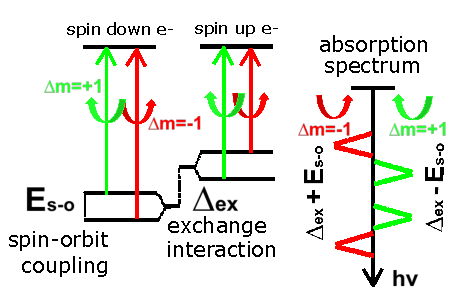
\includegraphics[width=150mm]{figs/XMCDMicroscopic.pdf}
\end{center}
\caption{Simplified electronic structure for the microscopic picture of X-ray magnetic circular dichroism. }
\label{XMCDMicroscopic}
\end{figure}

\section{Kerr Effect}

The microscopic origin for XMCD is identical to that of resonant magneto optical Kerr effect. This process simply employs the EUV light's sensitivity to the exchange splitting in a reflection geometry. The origin of the dielectric tensor that interacts with the incident light is the same as that outlined above. From here, we will treat the interaction of light with the dielectric tensor, since it provides a convenient way for computing magneto-optical effects (which can manifest themselves in a number of different ways depending on the geometry used).

When linearly polarized light reflects from a magnetized solid it is modified in two ways: first the direction of polarization is rotated over an angle $\Theta_K$, and secondly the phase of the light is modified so that it becomes elliptically polarized. When the magnetization is applied in a transverse geometry (see Fig. ref), the amplitude of the light is modified as well. It is this effect, that we will employ for the majority of the work in this thesis, due to the fact that changes in intensity are much simpler to monitor in the EUV light regime than changes in the polarization of the light.

\subsection{Transverse magneto-optical effect (TMOKE)}
 
We now consider the interaction of magnetic media magnetized in the transverse direction (see fig ref) with linearly polarized light. In the s- and p- polarization basis ($E_s$,$E_p$), we write the incident electric field $\vec{E_i}$, i.e. the time- and space- independent part of the (plane wave) radiation as

\begin{equation}
\overrightarrow{E_i} = \left({\begin{array}{c}
	E_s \\
	E_p \\
	\end{array} } \right) 
= \left({\begin{array}{c}
	\text{cos}(\theta) \\
	\text{sin}(\theta) \\
	\end{array} } \right) E_0
\end{equation}

with $E_0$ the amplitude of the incoming electric field vector. In the following, we set $E_0$ to 1. $\Theta$ is the angle of the linearly polarized radiation relative to the s-polarization direction. The reflected field $\overrightarrow{E_r}$ can be related to the incident field through the Fresnel reflection matrix $\hat{r}$ as

\begin{equation}
\overrightarrow{E_r} = \hat{r}\overrightarrow{E_i}=\hat{r}\left({\begin{array}{c}
	\text{cos}(\theta) \\
	\text{sin}(\theta) \\
	\end{array} } \right) .
\end{equation}

Now this matrix depends on the magnetization direction of the solid and can be written when $\vec{m}$ lies in the (x,y) plane as,

\begin{equation}
\hat{r}(\vec{m})= \left({\begin{array}{cc}
	r_{ss} & r_{sp} \\
	r_{ps} & r_{pp} \\ 
	\end{array} } \right) 
= \left({\begin{array}{cc}
	r_{ss}^{(0)} & r_{sp}^{(1)}m_y Q \\
	-r_{sp}^{(1)} m_y Q & r_{pp}^{(0)}+r_{pp}^{(1)}m_x Q \\ 
	\end{array} } \right)
\end{equation}

with the magneto-optical Voigt constant Q=i$\epsilon_{xy}$/$\epsilon_{xx}$ and the subscripts (0) and (1) indicate the coefficients in terms independent and linear in Q, respectively. Note that for the special case of the magnetization lying entirely in the x direction, the dielectric tensor will cause only the p-polarized light to be directly affected by the magnetization. In this work and many others, it is common to define an experimentally measurable quantity, the magnetic asymmetry:

\begin{equation}
A=\frac{R_+ - R_-}{R_+ + R_-}
\end{equation}

where $R_+$ is the reflected intensity when the sample is fully magnetized in one direction (arbitrary), and $R_-$ the reflected intensity when the sample is fully magnetized in the other direction. When the magnetization lies only along the x-direction ($m_x$=1, $m_y$=0), then the asymmetry depends on the angle of incidence of the light and the material's Voigt constant as:

\begin{equation}
A = \frac{m_x(1-\cos{2\theta})\text{Re}(r_{pp}^{(0*)}r_{pp}^{(1)}Q)}{|r_{pp}^{(0)}|^2\sin^2{\theta}+|r_{ss}|^2\cos^2{\theta}}
\end{equation}


\section{High Harmonic Generation}

\section{Details of Experimental Setup}
For the Tr-TMOKE experiments, the experimental layout is given in Fig \ref{fig: NiSIfig1}C. A regenerative Ti:Sapphire amplifier system is used to generate pulses of up to 1.8 mJ at a repetition rate of 5 kHz. The beam is then split with a 10:1 beamsplitter for use in the pump/probe configuration. The probe beam is focused with a 50 cm lens into a hollow core fiber with a diameter of 150 $\mu$m. The hollow core fiber is filled with He gas at a pressure of 1 Torr, where high harmonics of the fundamental beam are generated. After the harmonics are generated, the beam passes through an iris to remove some of the residual fundamental mode, is reflected by a toroid with an effective focal length of 30 cm, and passes through an aluminum filter of thickness 500 nm. Next, the harmonic beam is rejoined by the p-polarized pump beam, and the two are incident on the sample at an angle of 48 degrees measured with respect to the normal. The timing of the pump beam with respect to the probe is controlled by a mechanical delay stage. The power in the pump arm is controlled by a polarizer and mechanical half waveplate combination (for fluence dependent studies). The FWHM of the pump pulse for both the TMOKE and reflectivity measurements at the location of the sample was determined to be 55 fs by in-situ frequency resolved optical gating measurements. After reflecting off the sample, the HHG probe reflects off a grating (500 lines/mm) placed in the conical mount configuration and passes through two more aluminum filters of thickness 200 nm before being measured by an Andor Newton X-ray CCD detector.

